\qrchapter{https://forgottenpillar.com/rsc/en-fp-chapter4}{Revision of “Living Temple”}


\qrchapter{https://forgottenpillar.com/rsc/en-fp-chapter4}{Marekebisho ya “Living Temple”}



Katika \textit{Testimonies for the Church containing Letters to Physicians and Ministers Instruction to Seventh-Day Adventist}, sura ya kumi, \textit{Msingi wa Imani yetu,} Mungu alitoa masomo ya thamani kuhusu uendelezaji na matokeo ya nadharia za Kellogg. Maana ya kina ya dondoo hizi zinaweza kueleweka tunapofahamu muktadha wao ya kihistoria. Hebu kwanza tuangazie kwa ufupi muktadha wa kihistoria wa kitabu cha Kellogg, The \textit{Living Temple}.


Kwa majaliwa, Mungu alionyesha kwamba “\textit{Living Temple}” haipaswi kuchapishwa. Matukio ya ajabu kama vile kuchomwa kwa jengo la waandishi wa habari la Battle Creek, usiku wa kuamkia siku ya kuchapishwa, yalitokea. Hatimaye, kitabu hicho kilichapishwa mahali pengine; kitabu kilizua mgogoro mkubwa katika Kanisa la Waadventista Wasabato. Mnamo Oktoba 7, 1903, mkutano wa kila mwaka wa Conference ulifanyika Washington DC. Viongozi wengi wa kanisa la Waadventista Wasabato walikuwepo, wakiwemo Dk. Kellogg na wafuasi wake. Mabishano makubwa yalikuwa yakifanyika juu ya kitabu hiki na mzozo haukuepukika. Kwa bahati nzuri, wakati mgogoro huu ulichacha sana, barua kutoka kwa Dada White iliwasilishwa kwa baraza. Siku ya Jumapili, barua hiyo ilianguka kwenye masikio ya wote, na kutokana nayo, zilisikika “amina” na “haleluya” nyingi. Ilikuwa asubuhi yenye wasiwasi na yenye kusisimua kwa ajili ya kanisa lililokuwa karibu kugawanyika—hatimaye kuwa na mwelekeo thabiti kutoka kwa Mjumbe wa Bwana:


\begin{figure}[h]
    \centering
    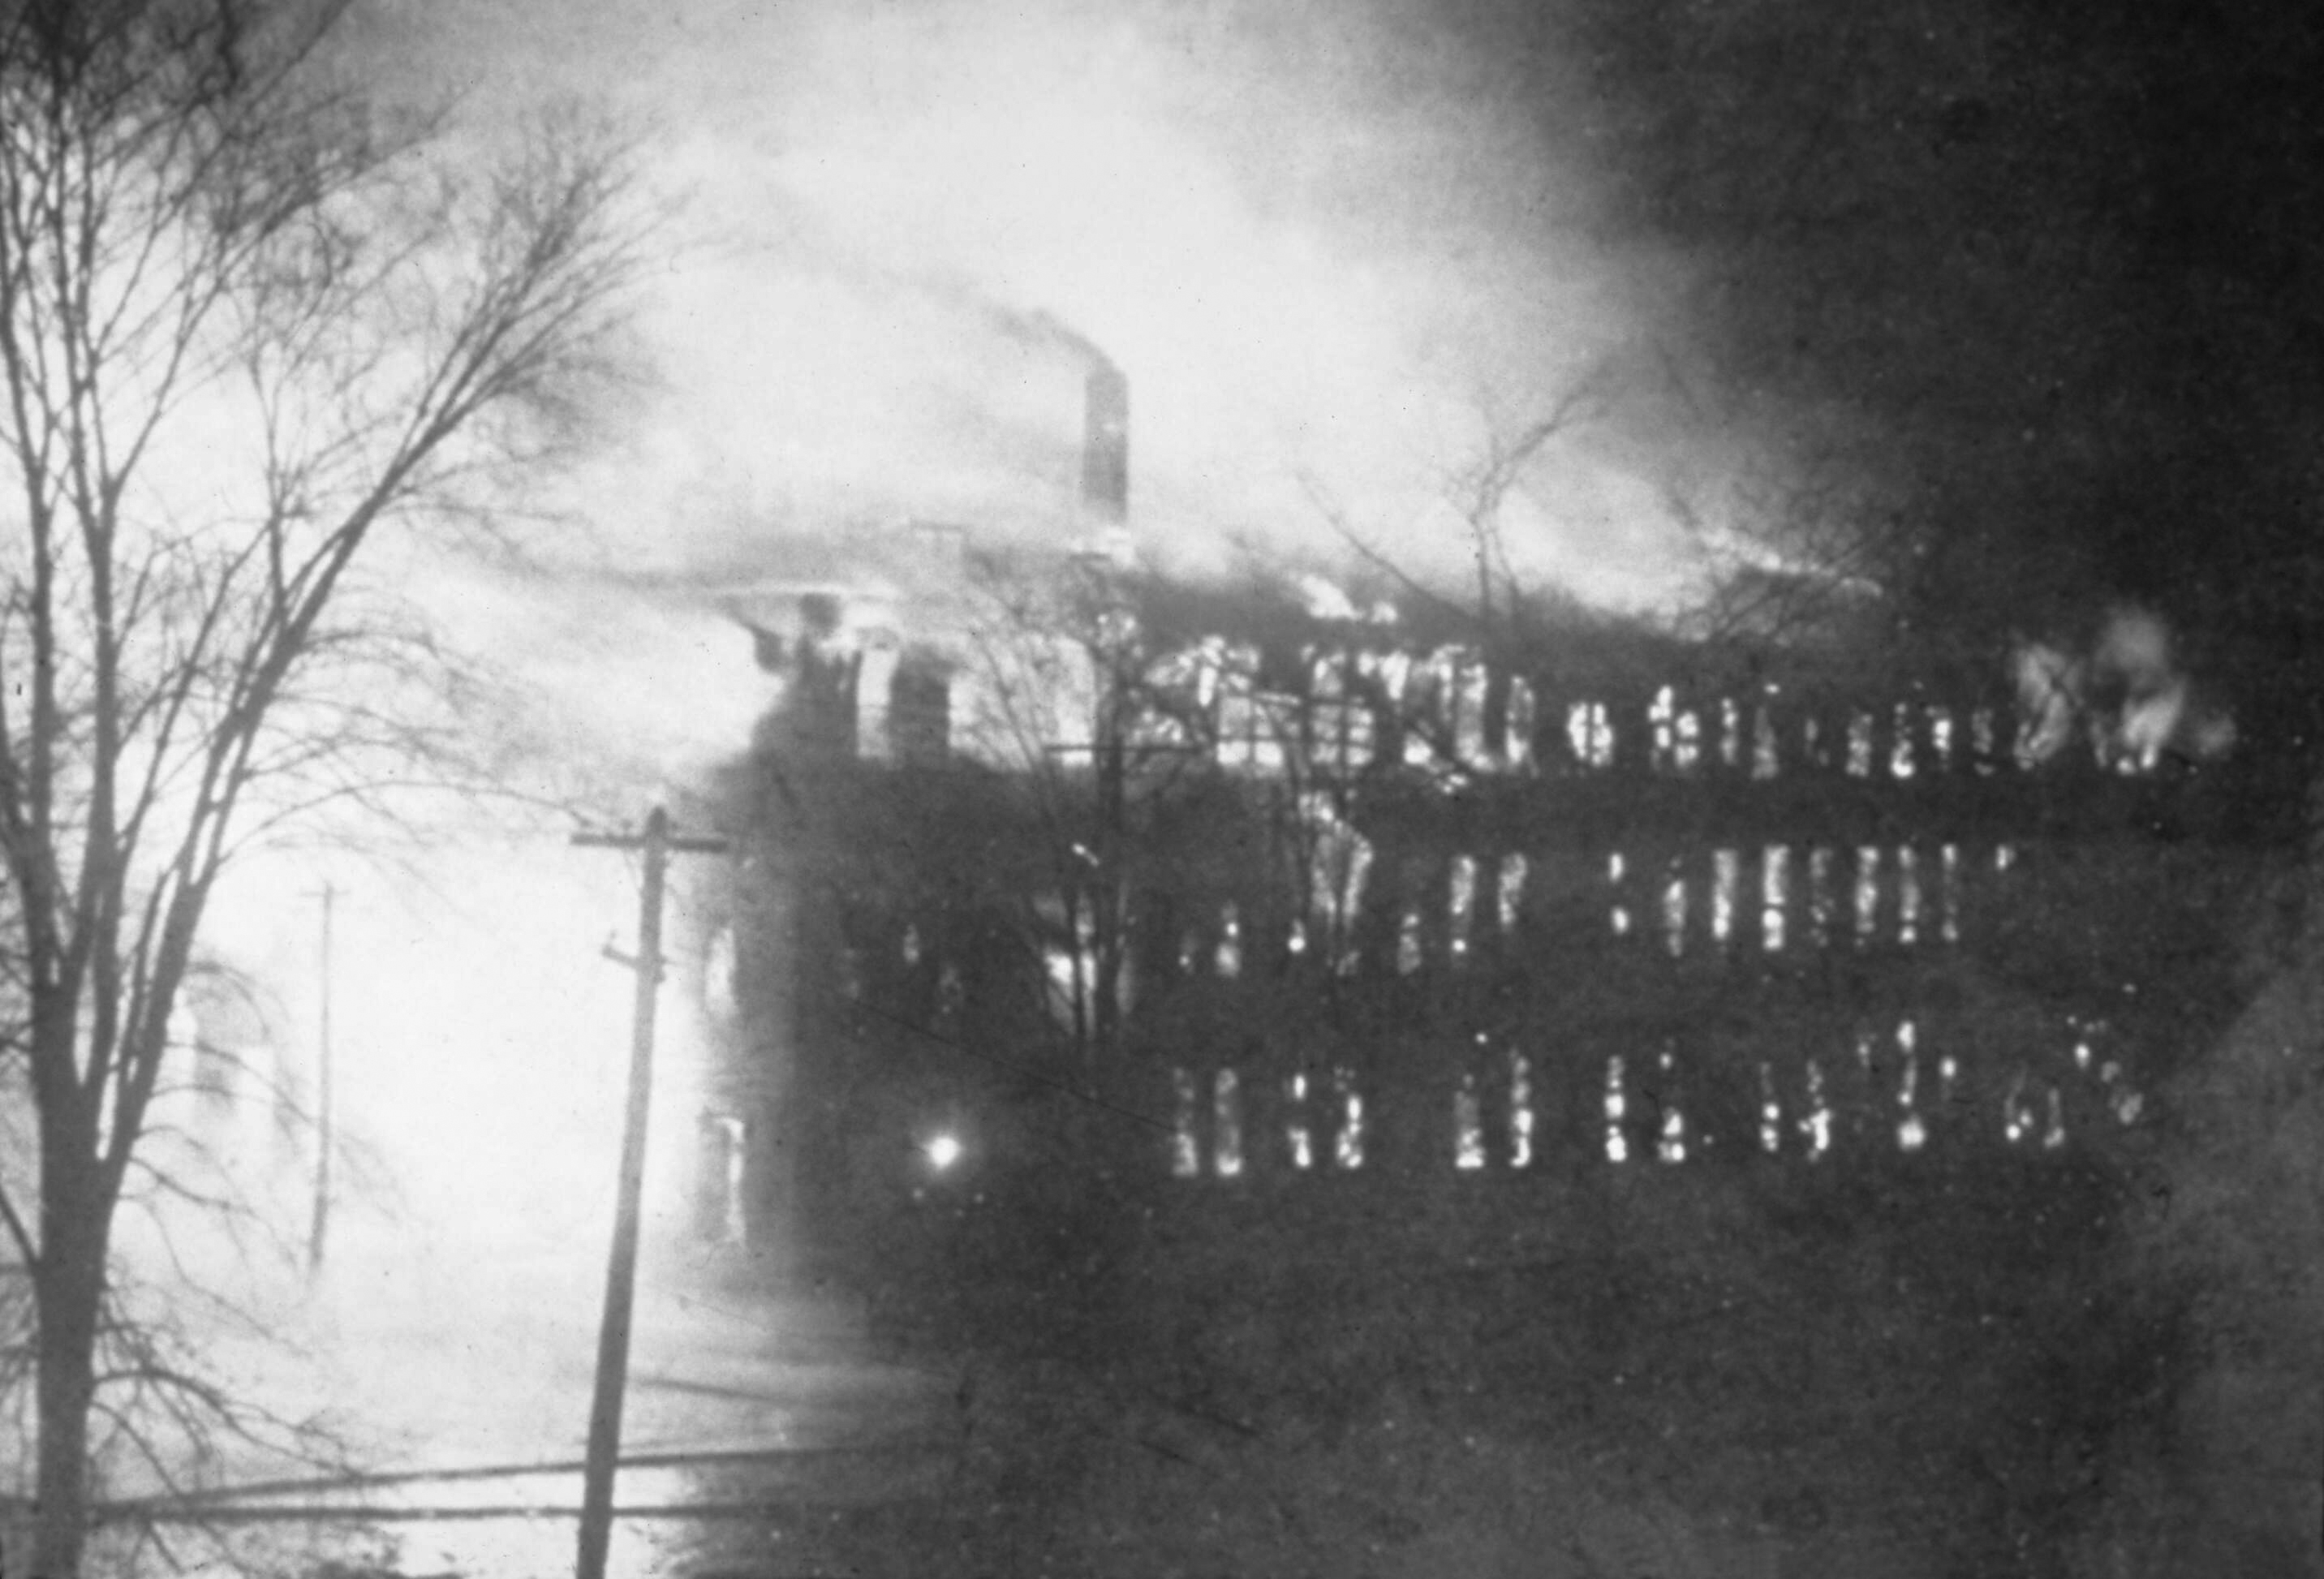
\includegraphics[width=1\linewidth]{images/review-and-herlad.jpg}
    \caption*{Burning of Review and Herald press building, December 30, 1902.}
    \label{fig:review-and-herald}
\end{figure}


\begin{figure}[h]
    \centering
    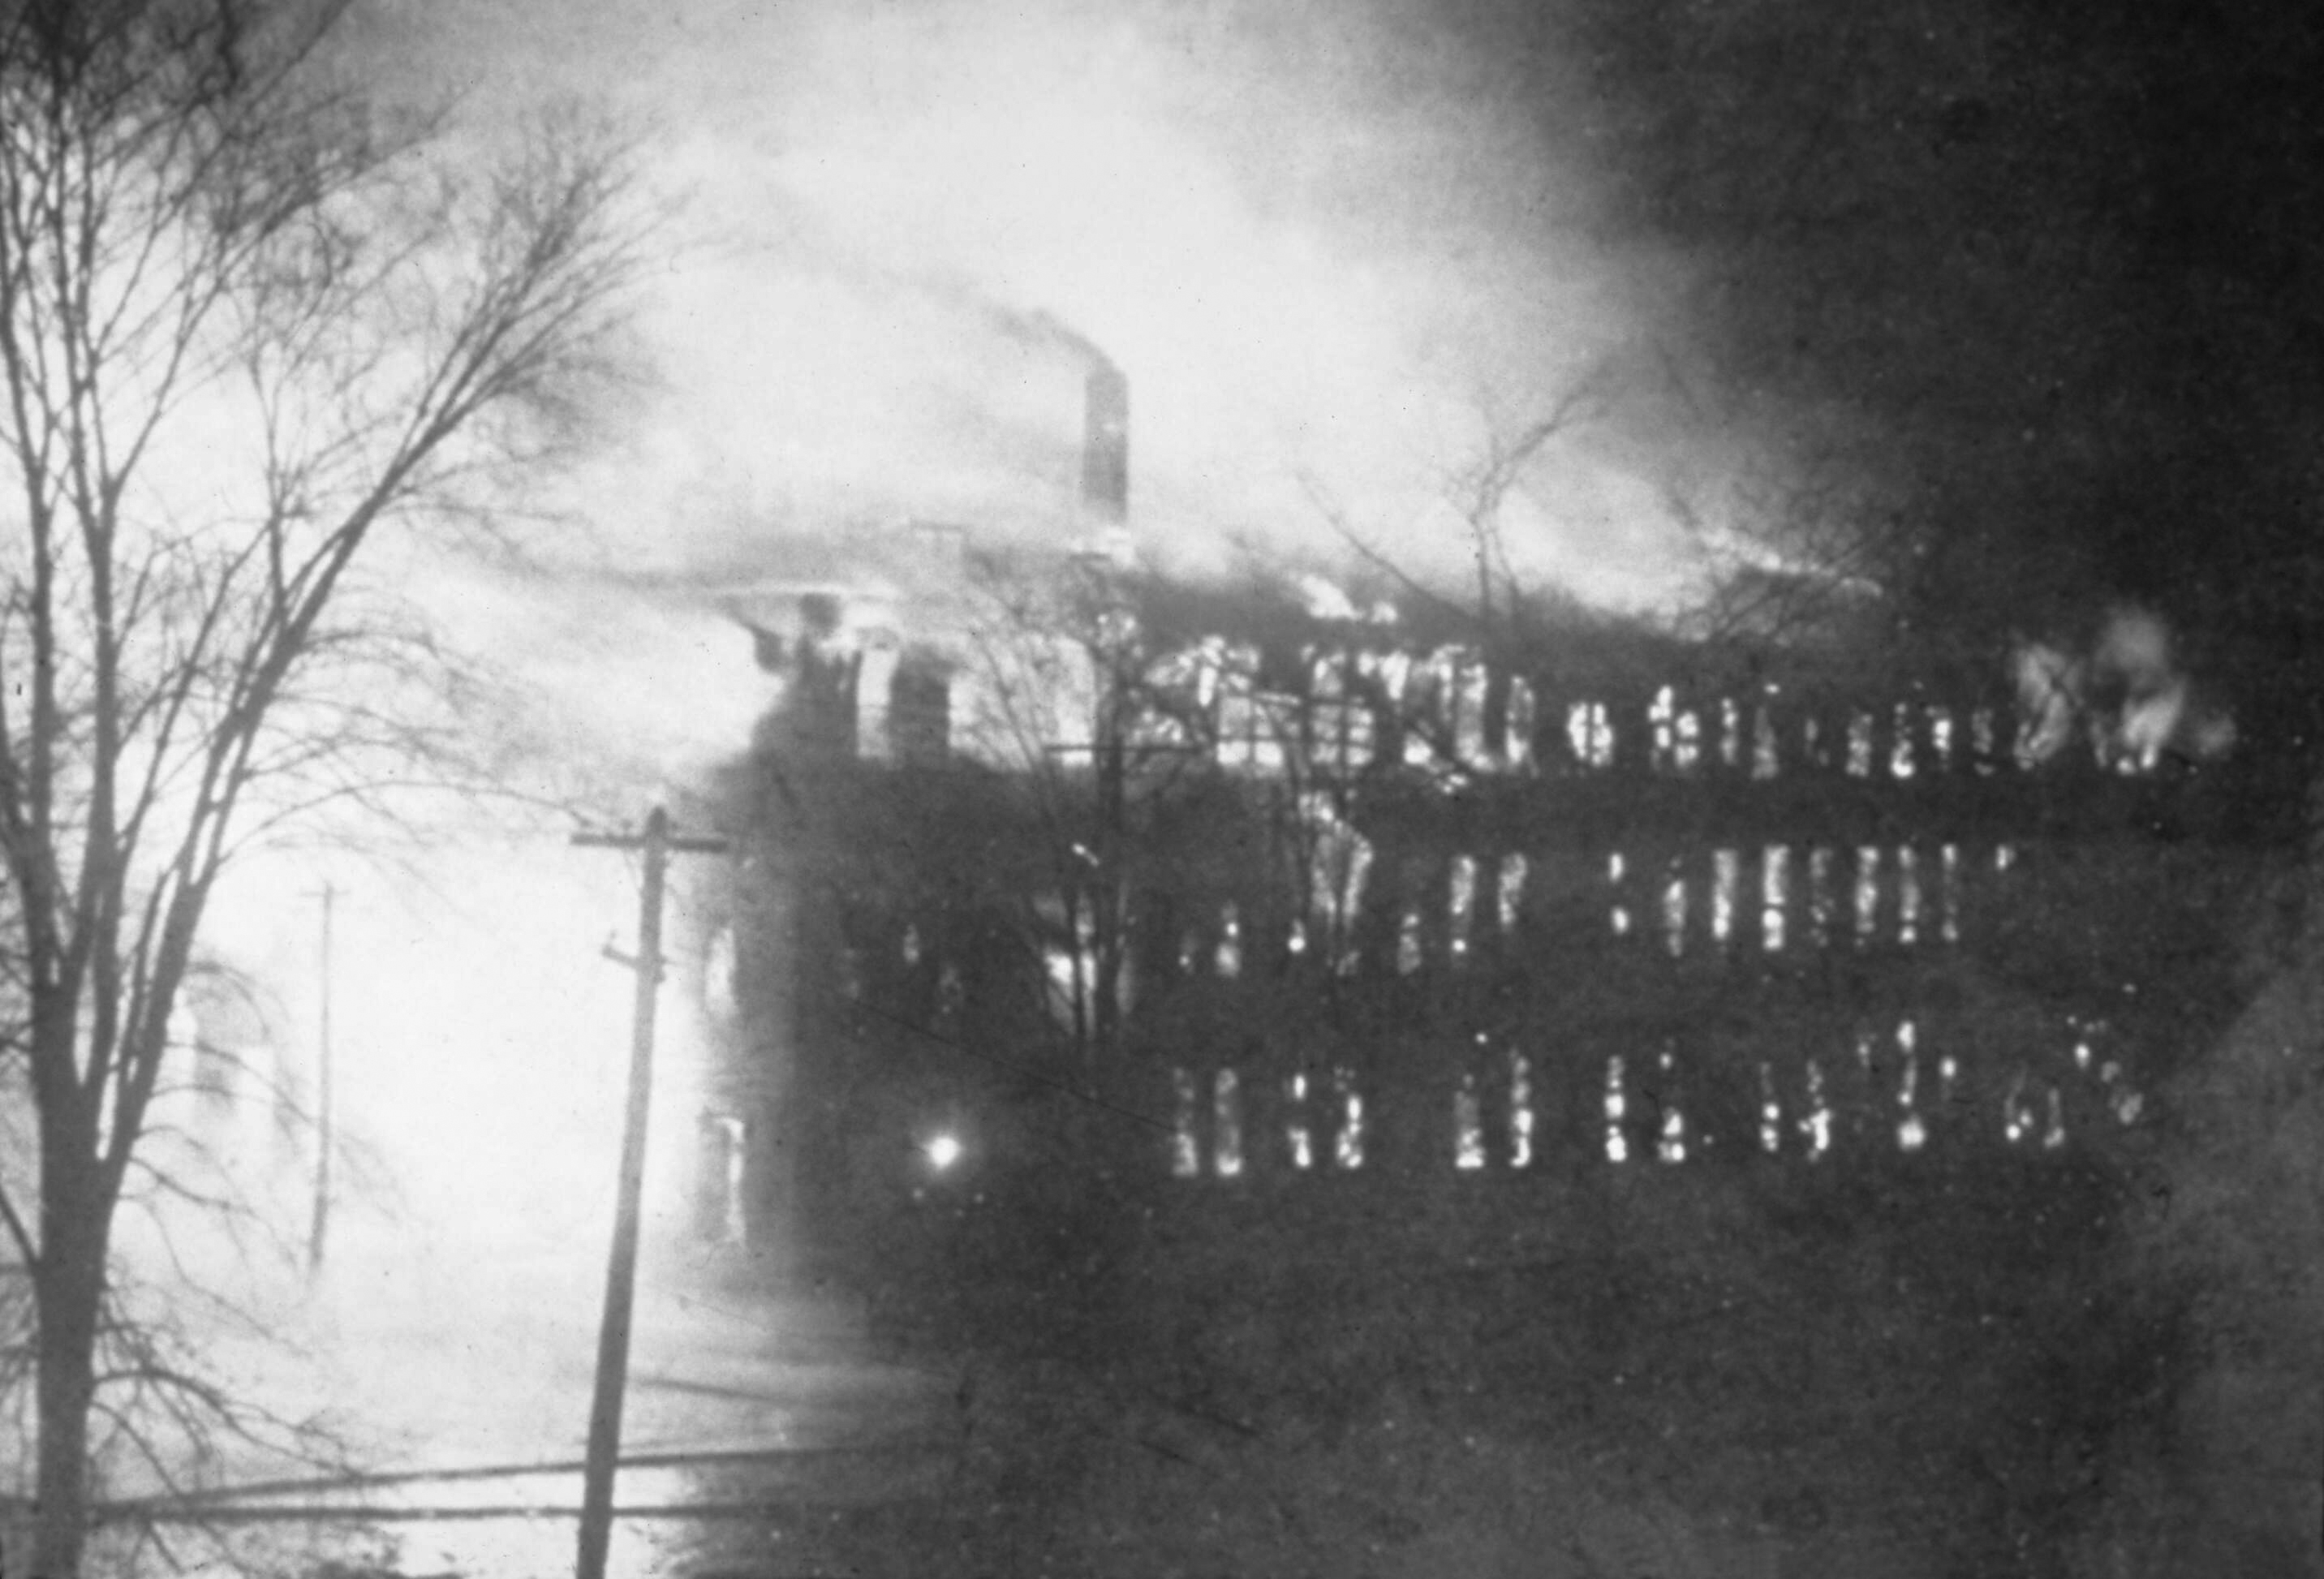
\includegraphics[width=1\linewidth]{images/review-and-herlad.jpg}
    \caption*{Kuchomwa kwa jengo la uchapishaji la Review and Herald, Desemba 30, 1902.}
    \label{fig:review-and-herald}
\end{figure}



\egw{Nina mambo fulani ya kuwaambia walimu wetu kuhusiana na \textbf{kitabu kipya The Living Temple}. \textbf{Kuwa mwangalifu jinsi unavyodhibitisha hoja za kitabu hiki kuhusu \underline{ubinafsi wa Mungu}}. Kulingana na yale ambayo Bwana amewasilisha kwangu, \textbf{hoja hizi hazina uthibitisho wa Mungu}. \textbf{Ni mtego ambao adui ameweka katika siku hizi za mwisho}. Nilifikiri kwamba hii ingetambuliwa na kwamba haingenilazimu kusema lolote. \textbf{Lakini kwa vile madai yametolewa kuwa mafundisho ya kitabu hiki yanaweza kudumishwa na maandishi yangu, ninalazimika kuongea ili kukana madai haya}. Kunaweza kuwa katika kitabu hiki misemo ambayo inapatana na maandishi yangu. Na kunaweza kuwa katika maandishi yangu kauli nyingi ambazo zikitolewa kwenye miktadha yao, na kufasiriwa kulingana na mawazo ya mwandishi wa Living Temple, zingeonekana kuwa zinapatana na mafundisho ya kitabu hiki. \textbf{Hii inaweza kutoa dhana kuwa hoja za Living Temple zinapatana na maandishi yangu}. \textbf{Lakini Mungu azuie ushindi wa maoni haya}.}[Lt211-1903.1; 1903][https://egwwritings.org/read?panels=p14068.9598008]



Mara kwa mara, Dada White alisema kwamba tatizo la kweli la kitabu hicho lilikuwa maoni\egwinline{\textbf{kuhusu ubinafsi wa Mungu}}. Maoni haya haziungwi mkono na kauli kutoka kwa maandishi ya Ellen White na maoni zizi hizi\egwinline{\textbf{ni mtego ambao adui ametayarisha kwa siku hizi za mwisho}}.


Mungu, tena katika majaliwa yake, alitatua mgogoro huu. Kellogg alikubali karipio kutoka kwa mjumbe wa Bwana na, kabla ya baraza kufungwa, alisema kwamba Living Temple ingetolewa sokoni\footnote{\href{https://forgottenpillar.com/wp-content/uploads/2022/04/Letter-A-G-Daniells-to-W-C-White-October-29-1903.pdf}{Letter: A. G. Daniells to W. C. White, October 23, 1903, pp. 5}}. Lakini baada ya mkutano huo, alizungumza faraghani na rais wa mkutano mkuu, Ndugu Arthur G. Daniells, kuhusu mipango yake ya kurekebisha kitabu hicho. Tutaangazia barua kadhaa zinazofichua mipango ya Kellogg ya kurekebisha “\textit{Living Temple}”.


Ellen White hakuwepo katika mkutano wa kila mwaka huko Washington DC lakini mwanawe, William C. White, alihudhuria. Mkutano ulipoisha, ndugu Arthur G. Daniells aliandika barua ya siri kwa William C. White kuhusu mpango wa Dk. Kellogg wa kurekebisha kitabu chake:



\others{Oktoba 29, 1903}




\othersnogap{Tangu \textbf{baraza lilipofungwa} nimeona nikuandikie \textbf{kwa siri kuhusiana na mipango ya Dk. Kellogg ya kurekebisha na kuchapisha upya ‘The Living Temple’}…. Yeye \normaltext{[Kellogg]} alisema kwamba siku kadhaa kabla ya kufika kwenye baraza, alikuwa akitafakari jambo hilo, na alianza kuona kwamba \textbf{alifanya makosa kidogo katika kutoa maoni yake}. Alisema wakati huo wote wa kucharaza hisia zake ametatizika kujua jinsi ya kutaja  uwepo wa Mungu na vile vile jinsi Mwenyezi anahusiana na kazi zake za uumbaji...}


\begin{figure}[hp]
    \centering
    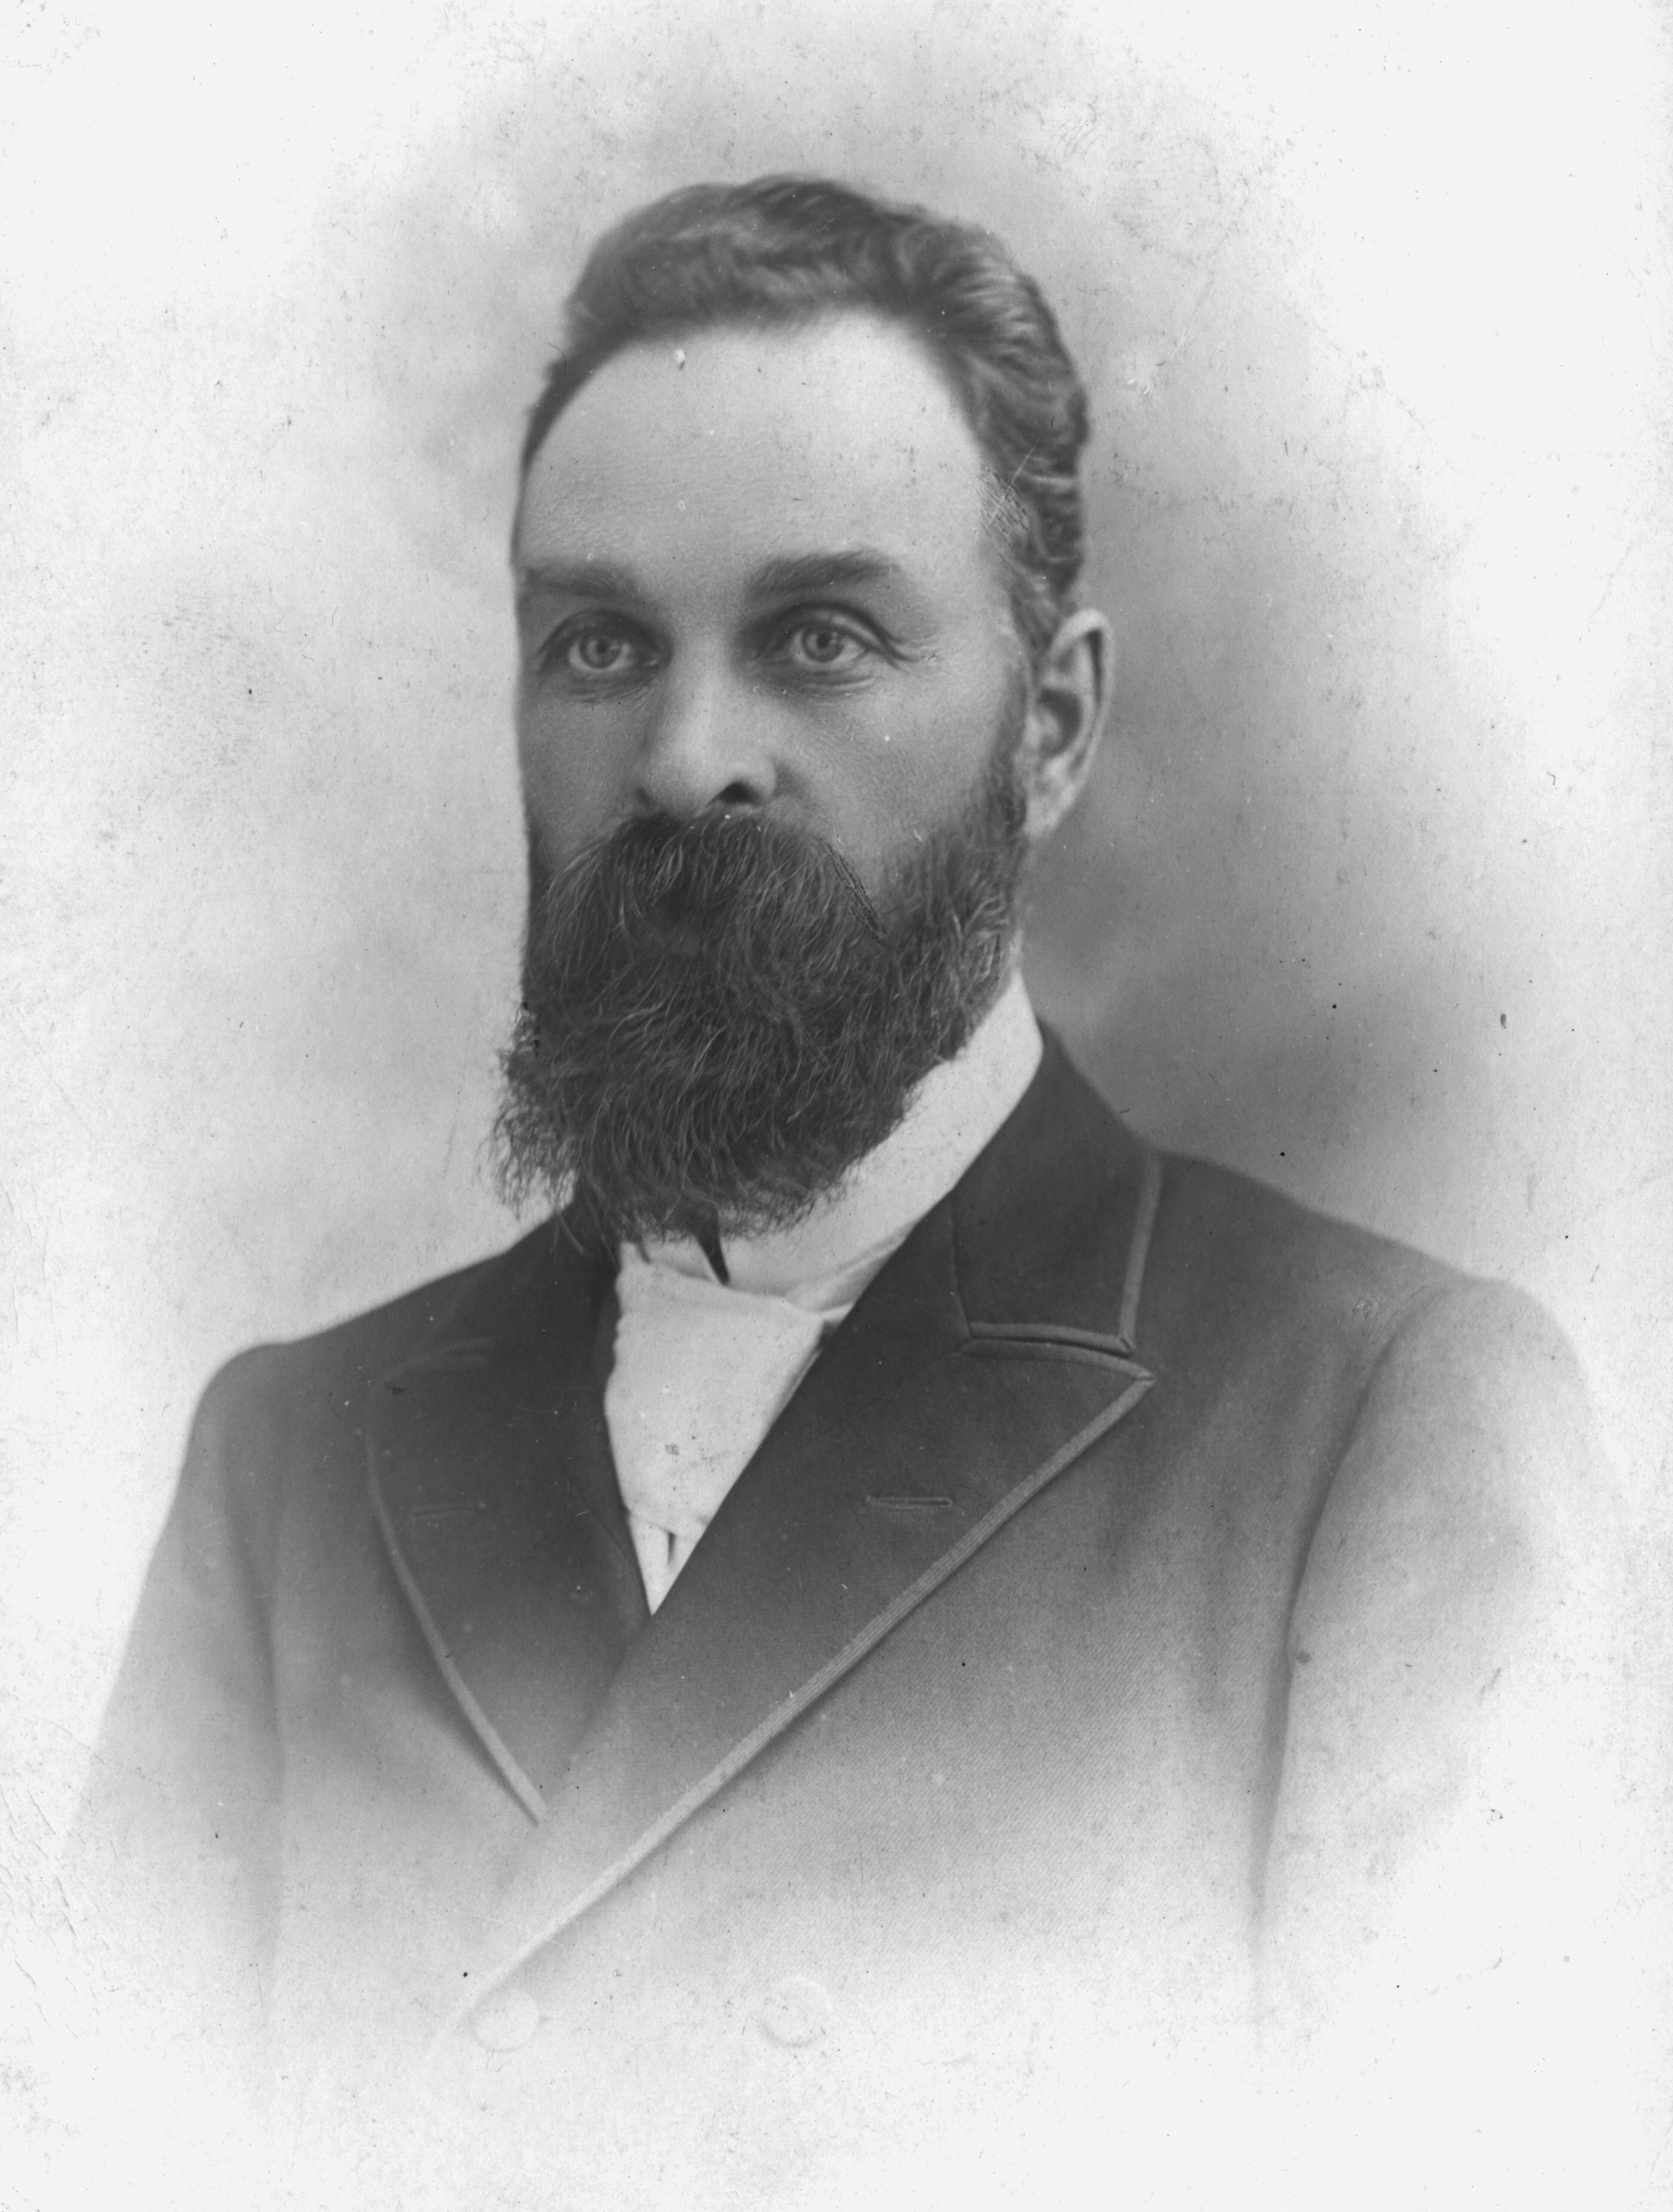
\includegraphics[width=1\linewidth]{images/daniels.jpg}
    \caption*{Arthur Grosvenor Daniells (1858-1935)}
    \label{fig:daniells}
\end{figure}


\begin{figure}[hp]
    \centering
    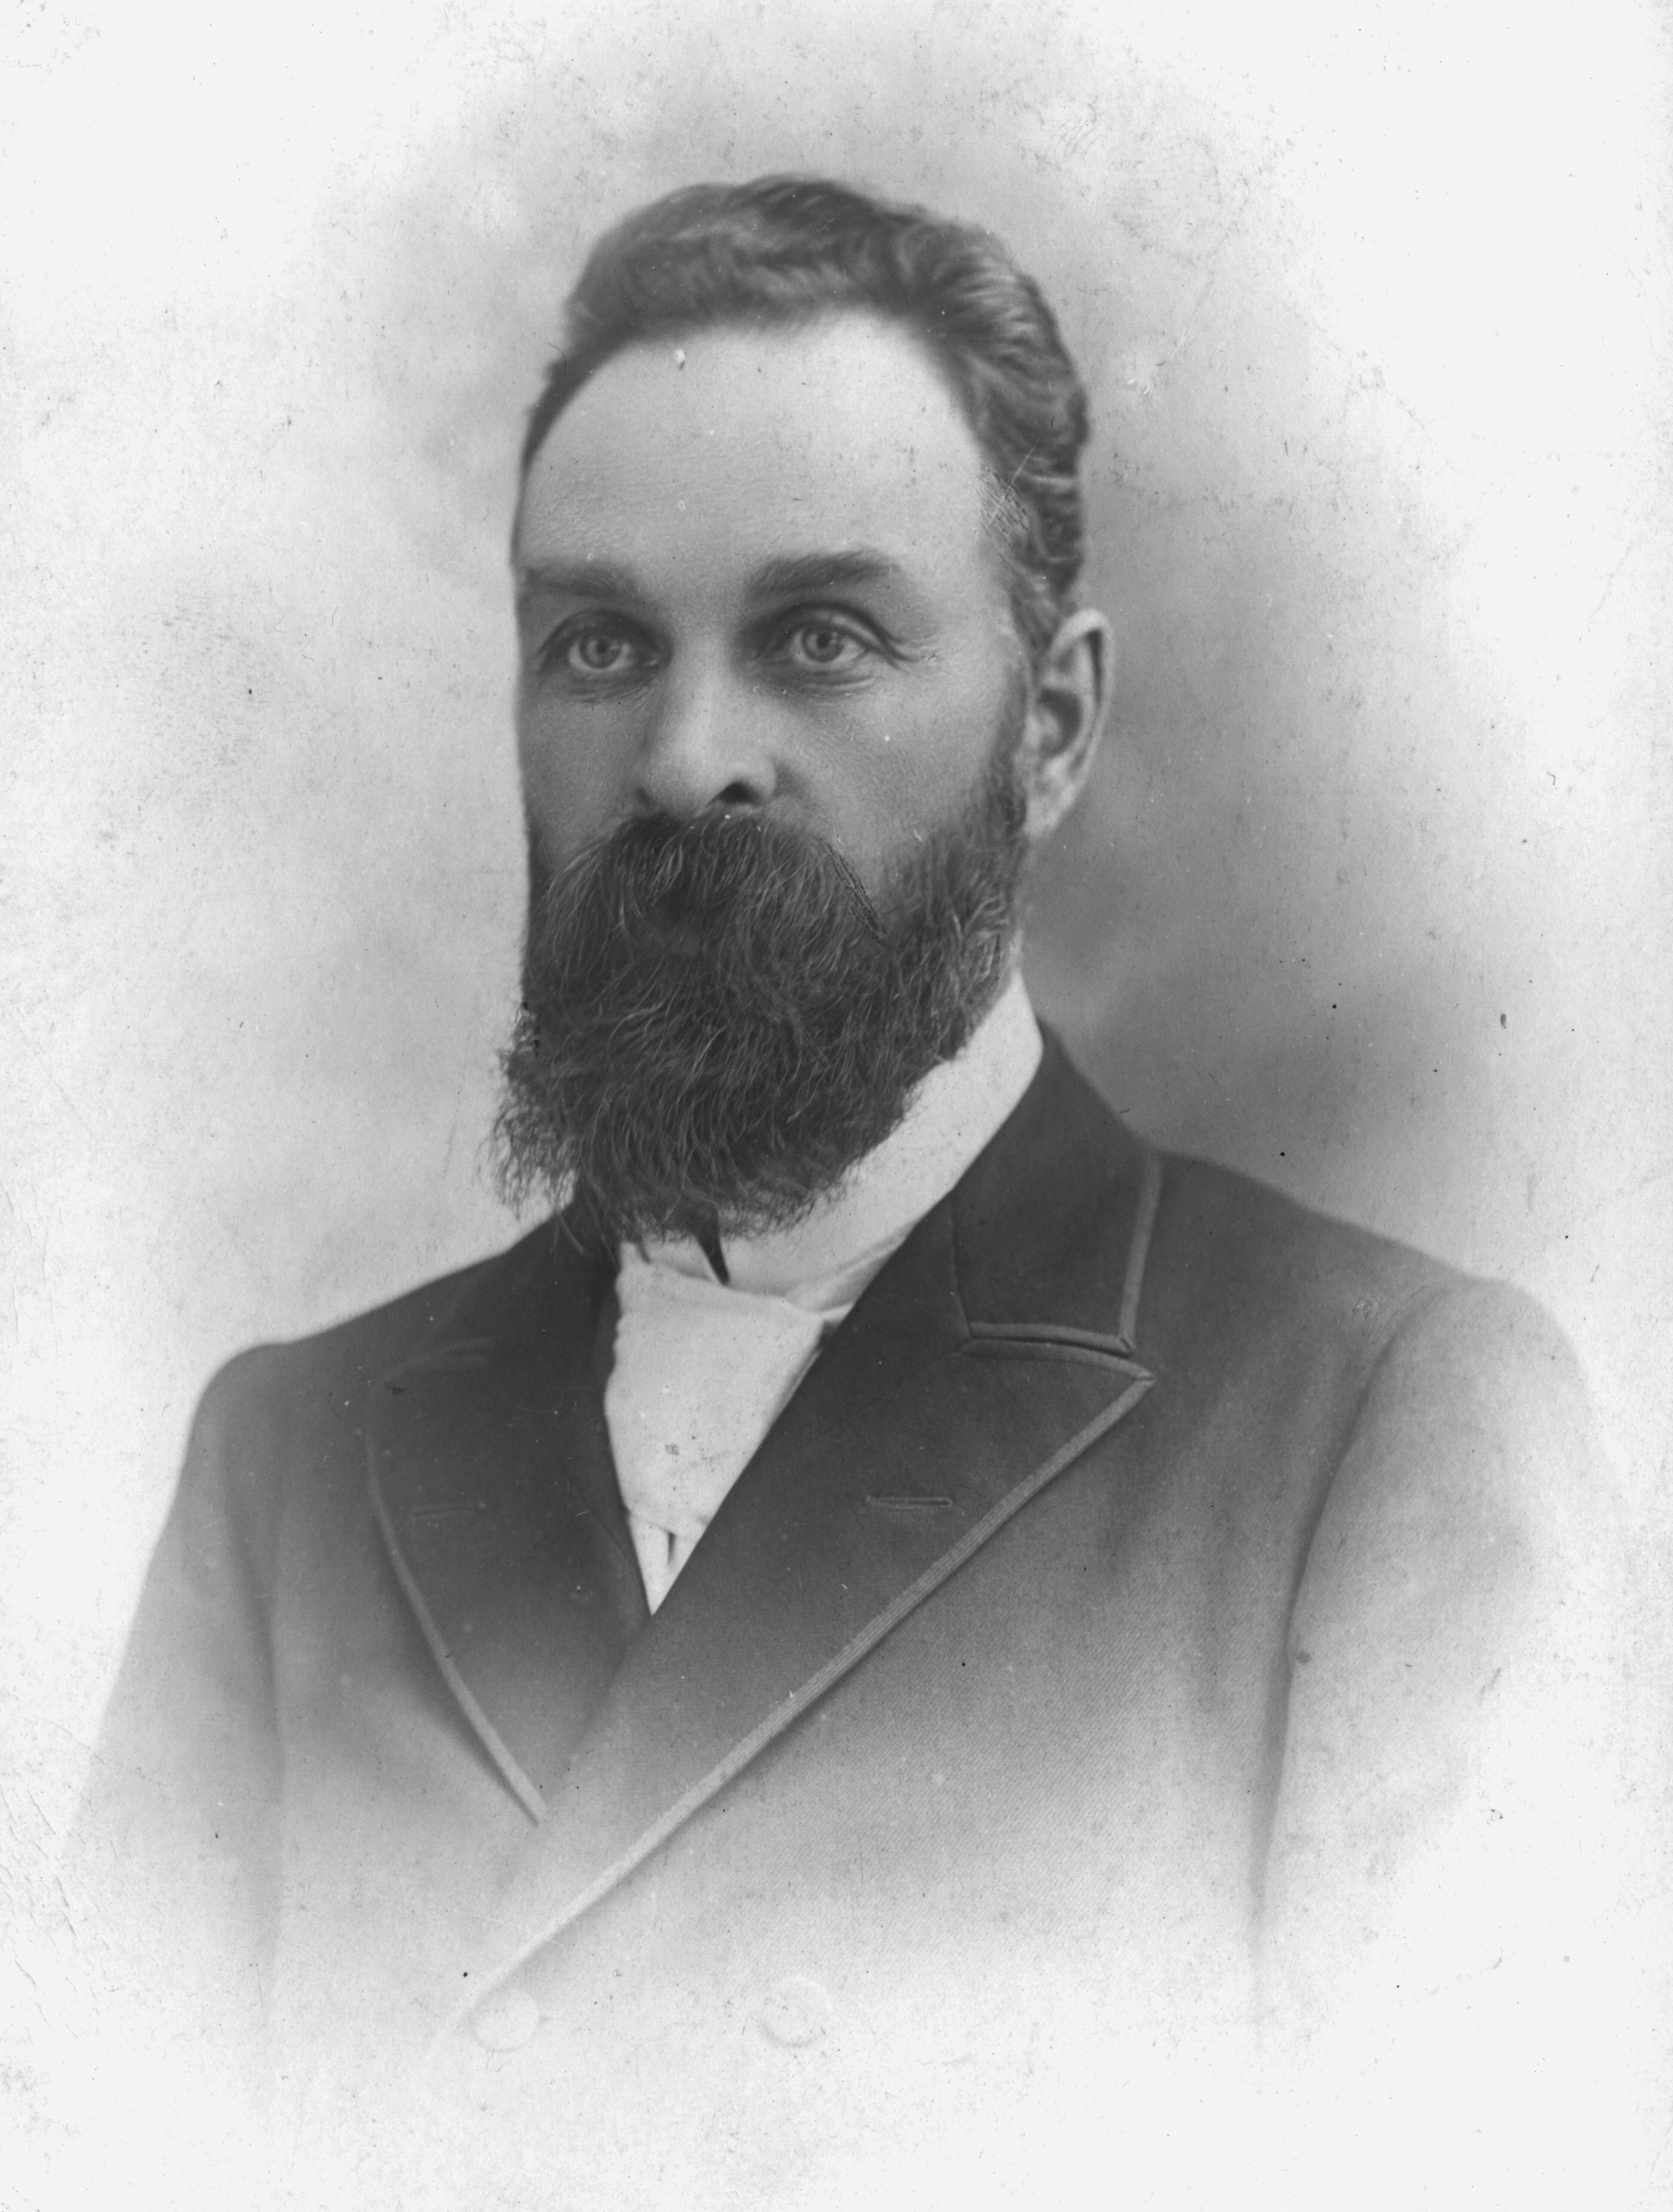
\includegraphics[width=1\linewidth]{images/daniels.jpg}
    \caption*{Arthur Grosvenor Daniells (1858-1935)}
    \label{fig:daniells}
\end{figure}



\othersnogap{\textbf{Kisha akasema kwamba maoni yake ya awali \underline{kuhusu utatu} yalikuwa yamemzuia kutoa kauli iliyo wazi na sahihi kabisa; lakini kwa muda mfupi \underline{amekuwa mwaminifu katika fundisho la utatu} na kwa hivyo kwa wakati huu anayo mtazamo toshelezi kung'amua bila tashwishi pale ambapo ugumu wote ulikuwa, na aliamini kwamba angeweza kusuluhisha jambo hilo kwa njia ya kuridhisha.}}



\othersnogap{\textbf{Aliniambia kwamba sasa anaamini katika \underline{Mungu Baba, Mungu Mwana, na Mungu Roho Mtakatifu}; na maoni yake yalikuwa kwamba ilikuwa ni Mungu Roho Mtakatifu, na si Mungu Baba, aliyejaza nafasi zote, na kila kiumbe lililohai. Alisema angeliamini \underline{hili} kabla ya kuandika kitabu, angeweza kutoa maoni yake bila kutoa maoni ya-siyofaa jinsi kitabu sasa kinatoa.}}



\othersnogap{\textbf{Niliweka mbele yake pingamizi nilizozipata katika mafundisho hayo, na kujaribu kumwonyesha hiyo mafundisho yalikuwa kinyume kabisa na injili na hivi kwamba sikuona jinsi inavyoweza kurekebishwa kwa kubadilisha misemo michache tu.}}



\othersnogap{Tulibishana katika suala hilo kwa muda fulani kwa njia ya kirafiki; lakini nilihisi kuwa, tulipoachana, daktari hakujielewa mwenyewe, wala kiini cha mafundisho yake. Na sikuweza kuona jinsi gani itawezekana kwa yeye \textbf{kubadilisha kikamilifu na kwa wakati wa siku chache \underline{kurekebisha kitabu} ili maoni yaliyowasilishwa yawe sawasawa}.}[Letter: A. G. Daniells to W. C. White, October 29, 1903. pp. 1, 2][https://forgotten-pillar.s3.us-east-2.amazonaws.com/Letter-A-G-Daniells-to-W-C-White-October-29-1903.pdf]


Kellogg hakuona kosa katika maoni yake; bali, katika kueleza maoni yake. Hakung'amua fika kwamba maoni yake yalikuwa ya uwongo, bali ni usemi wake tu wa maoni hayo, ambayo yalisababisha kitabu kutoa dhana potofu. Walakini, ni wazi, hii haikuwa kweli. Kama Dada White alivyosema, Kellogg alikuwa na tatizo kuhusiana na dhana ya \emcap{Umbile la Mungu} na pale Uwepo wake ulipo. Kwa hivyo, Kellogg alipendekeza kwamba ili “\textit{kurekebisha vitabu}” atajumuisha semi za utatu kwa sababu sasa alianza kuamini \textit{fundisho la Utatu}. Kwa wakati huu, Kanisa la Waadventista Wasabato halikuwa waamini wa fundisho la utatu—fundisho la Utatu halikuwa mojawapo ya vipengele vya \emcap{Kanuni za Kimsingi}, kama tulivyoona hapo awali. Hivyo, haishangazi kwamba Ndugu Daniels alipinga na kukanusha fundisho la Utatu, akidai kwamba lilikuwa\others{kinyume kabisa na injili.} Kurekebisha kitabu, kwa kubadilisha misemo michache, haingebadilisha tatizo kuu la kitabu: dhana zilizowasilishwa juu ya \emcap{Umbile la Mungu}.


Katika matukio yaliyoelezwa, na katika jibu la William White kwa Ndugu Daniells, tunaweza kuona kwa nini Dada White aliandika Shuhuda Maalum. William White alimjibu Kaka Daniells mnamo Novemba 4, 1903:


\others{Ndugu mpendwa, --}


\othersnogap{\textbf{\underline{Mama pamoja nami} tumesoma sasa hivi barua yako ya \underline{Oktoba 29} ambayo unazungumzia \underline{mipango mbalimbali ambayo imependekezwa kwa ajili ya kusahihishwa na kuchapishwa upya kwa ‘Hekalu Hai.’}}}


\othersnogap{Tulishangazwa sana na tangazo kwamba Dk. Kellogg angeondoa hiki kitabu kutoka kwenye soko ya vitabu, \textbf{na tunahuzunishwa kwa kweli kwa kuwa dhamira yake yanaelea kurudia mpango wa kukirekebisha kitabu hicho, \underline{Mama anajieleza kwa mkazo kabisa kuhusiana na jambo hili; anaiona kama kazi isiyo na faida}}. Nadhani atakuandikia hivi karibuni akitoa maoni yake kuhusu hili.}


\othersnogap{\textbf{… Naamini itakuwa muhimu \underline{kutoa Ushuhuda maalum hivi karibuni}, na huu lazima kujumuisha taarifa kamili na ya wazi kabisa kwa upande chanya wa swali hili, na pia makala zinazoonyesha makosa katika mafundisho ya wale ambao wamejitenga na ukweli kupitia nadharia za kuvutia na za udanganyifu}.}[\href{https://ellenwhite.org/letterbooks/555}{Barua kutoka W.C. White kwa A.G. Daniells, Nov. 4, 1903,} (uk. 458)]


\begin{figure}[h]
    \centering
    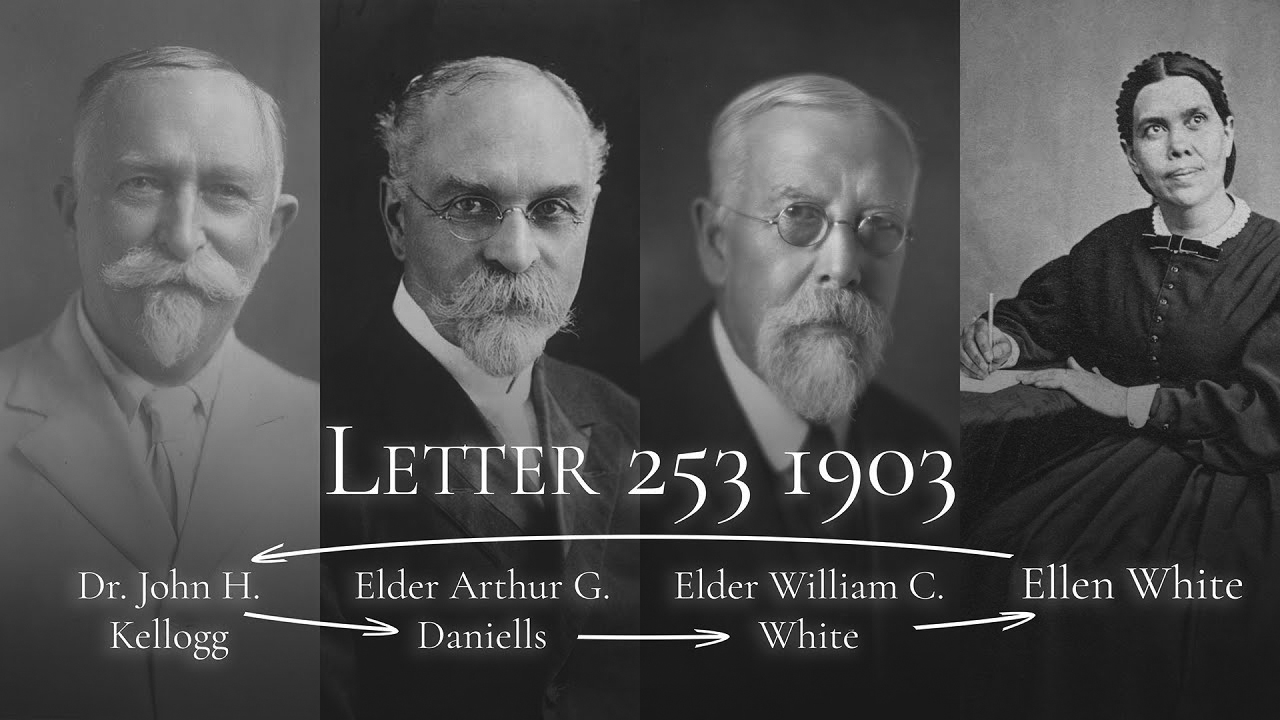
\includegraphics[width=1\linewidth]{images/correspondance.jpg}
    \caption*{Correspondence chain between A. G. Daniells, W. C. White, Ellen White and Dr. John H. Kellogg.}
    \label{fig:corespondance}
\end{figure}


\begin{figure}[h]
    \centering
    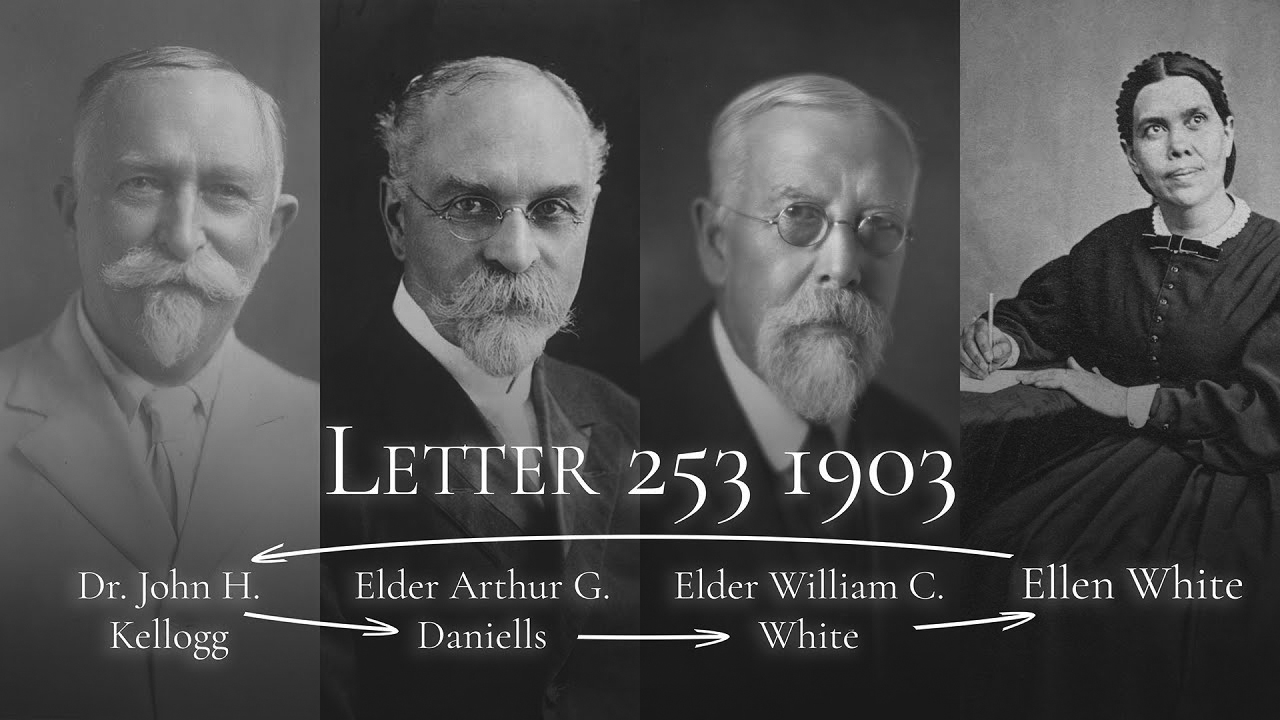
\includegraphics[width=1\linewidth]{images/correspondance.jpg}
    \caption*{Mfululizo wa mawasiliano kati ya A. G. Daniells, W. C. White, Ellen White na Dk. John H. Kellogg.}
    \label{fig:corespondance}
\end{figure}



Huu hapa ni ushahidi kwamba Dada White alikuwa anafahamu nia ya Dk. Kellogg ya kurekebisha “\textit{Hekalu Hai}” na kufahamiana kwake na imani yake katika Fundisho la Utatu. Kwa maneno ya William, yeye alijieleza kwa msisitizo kabisa kuhusiana na jambo hili. Aliona kuwa haina faida kufanya urekebisho. Kwa sababu hii, ilikuwa ni lazima kutoa Ushuhuda maalum hivi karibuni. Na vivyo ndivyo ushuhuda ulikuwepo. Hivi ndivyo \textit{Shuhuda za Kanisa zenye Barua kwa Madaktari na Maelekezo kwa Wahudumu kwa Waadventista Wasabato} ilichapishwa mwaka wa 1904, yenye barua kwa madaktari na wahudumu waliounganishwa na mgogoro wa Kellogg.


Kwa kusema \others{\textbf{\underline{Mama pamoja nami} tumesoma sasa hivi barua yako ya \underline{Oktoba 29}}}, William alithibitisha kwamba Dada White alijua kikamilifu nia ya Kellogg na imani yake kuhusu utatu. Baada ya yeye kusoma Barua ya Daniells, aliandika jibu la moja kwa moja kwa Dk. Kellogg. Barua hii ni \textit{Lt253-1903}. Ni barua maarufu sana na ya kufungua macho kwa sababu inafichua wazi jinsi nabii alivyoshughulika na Fundisho la Utatu. Aliinua fundisho juu ya \emcap{Umbile la Mungu} ulio wekwa katika \emcap{Kanuni za Kimsingi}. Kuna kufanana wa kushangaza kati ya barua hii na ya sura ya kumi ya Shuhuda Maalum, \textit{Msingi wa Imani yetu}.



% Revision of the Living Temple

\begin{titledpoem}
    
    \stanza{
        In Kellogg’s book, a subtle snare \\
        Though well-disguised through crafty care \\
        From Bible truth would lead away \\
        And cause some precious souls to stray.
    }

    \stanza{
        And though much scripture there was used \\
        The early truth became confused \\
        This error served to twist the mind \\
        But in God’s Word the truth we find.
    }

    \stanza{
        God’s personality has form \\
        To Bible truth we must conform \\
        On this the Doctor wasn’t clear \\
        But early Advent truth is dear
    }
    
\end{titledpoem}
